\chapter{Open Population Models}
\markboth{Open Populations}{}
\label{chapt.open}


\vspace{0.3cm}


\section{Introduction}


In the previous chapters we focused mostly on
 closed population models for
estimating density and for inference about spatial variation in
density.  However, a thorough understanding of population dynamics
requires information about both spatial and temporal variation in
population density and demographic parameters.  In this chapter, we
discuss modeling
 the processes governing
spatial and temporal dynamics, namely survival, recruitment, and
movement (migration, dispersal, etc...).  The ability to estimate
these parameters is critical to both basic and applied ecological
research (\cite{knape_deValpine:2012}. For example, testing hypotheses
about life history trade-offs requires accurate estimates of both
survival and fecundity (\cite{caswell:1989, nichols_etal:1994}).
Inference about density-dependent population regulation, which has
fascinated theoretical ecologists for well over a century, is likewise
best accomplished by studying the factors affecting survival and
fecundity, rather than the more common approach of modeling time
series data \citep{nichols_etal:2000}.  A mechanistic understanding of
population changes, which is essential for basic ecological and
conservation based questions, requires useful models of vital
rates. Furthermore, if we know how environmental variables affect
demographic parameters, we can make predictions about population
changes under different future scenarios. We can also assess the
sensitivity of parameters such as population growth rate to variation
in survival or fecundity. Although matrix population models are often
used for these purposes \citep{caswell:1989,saether_bakke:2000}, the
same objectives can be accomplished by computing posterior predictive
distributions as part of the MCMC algorithm.

The modeling framework we will develop in this chapter is based on a
formulation of the classical Cormack-Jolly-Seber (CJS) and Jolly-Seber
(JS) type models \citep{cormack:1964, jolly:1965, seber:1965} that are
amenable to modeling individual effects, including individual
covariates.  There is a long history of use of these models in
fisheries, wildlife, and ecology studies \citep{pollock_etal:1990,
  lebreton_etal:1992, pradel:1996, williams_etal:2002,
  schwarz_arnason:2005, gimenez:2007}.  Additionally, there have been
many modifications and developments of the CJS and JS models including
dealing with individuals that do have a well defined home range but
instead are moving through the sampled area (transients), dealing with
more than one site or state (multi-state models; states maybe
geographic units, reproductive stage, etc.), and addressing individual
movement through spatially implicit models.


For the first time, these models can fully
integrate the movement of individuals in the vicinity of the
trap array
%%%onto and off of the trap array
with their encounter histories to simultaneously estimate density,
survival, and recruitment in a spatial model.
For many species, such
as those that are rare or not often observed by researchers, this allows
inferences to be made about survival and recruitment without having
to physically capture individuals.
Additionally, another reason for
extending SCR models to open populations arises purely from a
sampling perspective.  Longer time periods are often needed to sample
rare or elusive species to ensure that enough captures and recaptures
are produced.  This extended time frame can quickly lead to violations
in the assumption of population closure.  For example, the European
wildcat study that was mentioned in Chapt. \ref{chapt.covariates} (see
\citet{kery_etal:2011} for details) was
conducted over a year-long period.  While the researchers in that
study used a closed population model, they did model variation in detection
as a function of time to account for seasonal variation in behavior. 
%% andy added the last phrase to above line
 Another approach would have been to use an
open population model (the spatial capture recapture open models had
not been developed at the time of the wildcat study, so we'll forgive
the authors for not having used this more appropriate model).

In this chapter, we present the traditional JS model and
the spatial version, demonstrating both with an example of mist-netting of ovenbirds,
which was also analyzed in Chapt. \ref{chapt.poisson-mn}.  Then we review the
traditional CJS, multi-state CJS, and then describe the spatial model.  In this
section, we will use a an example of American shad.  Finally, we end by discussing
some of the new approaches to dynamics of activity centers including correlated
movement and dispersal.



\subsection{Brief overview of population dynamics}

The most basic formulation of models for population growth stems from
an idea originally used in accounting, the balance sheet.  To gain a
mechanistic understanding of population dynamics, it is important to
understand four fundamental processes that drive population size:
births and immigrants (i.e., population ``credits'') and deaths and
emigrants (i.e., population ``debits'').  The population at time $t+1$
is a function of these four components:
\[
N(t+1) = N(t) + B(t) + I(t) - D(t) - E(t)
\]
where $N(t)$ is the population size at time $t$, $B(t)$ and $I(t)$ are
the credits (additions) from births and immigrants at time $t$, and
$D(t)$ and $E(t)$ are the debits (losses) due to deaths and
emigration.  This balance equation model is known as the ``BIDE
model''.  A simple population growth model under density independence,
assuming no immigration or emigration, can be derived as:
\[
N(t+1) = N(t) + N(t)r(t)
\]
where $r(t) = b(t) - d(t)$.  Here, $b(t)$ and $d(t)$ are the
per-capita birth and death rates and thus $r(t)$ is the per-capita
growth rate. Models which are based only on the intrinsic population
growth rate, `r'; however, do not retain much information about the
underlying drivers of the population dynamics.  Density-dependent, age
structured, stochastic effects on growth, spatially structured, and
competition models (e.g., Lotka-Volterra) all are derivations of the
basic BIDE model.

In closed population models, we focus on estimating the population
size, $N$, but in open population models we are interested in the
dynamics that arise between years or seasons and thus we focus not
only on $N(t)$ but on the processes that drive the population changes.
By taking the basic parameters in the BIDE model and reconceptualizing
them, they can then be related to the commonly used parameters in JS
and CJS models, described in more detail throughout this chapter. In
the absence of movement, deaths (D) can be estimated in the CJS model
and both D and B (births) can be estimated in the JS model.  However,
in considering movement, it becomes difficult to distinguish births
from immigrants and deaths from emigrants. For example, survival
($\phi(t)$) is defined as the probability of an individual surviving
from time $t$ to $t+1$, and often this is called `\textit{apparent}
survival' because deaths and emigration cannot be
separated. Mortality, the probability of dying from time $t$ to $t+1$,
is $1-\phi(t)$.  Recruitment ($\gamma$) is the probability of a new
individual entering the population between $t$ to $t+1$, which
includes both those born into the population and immigrants. This
inability to distinguish between the different forms of losses and
gains does not allow researchers to test specific hypotheses about
population dynamics.  To address this, \cite{nichols_pollock:1990}
applied the robust design to a two age class situation in order to
separate estimates of recruitment into immigration and {\it in situ }
reproduction.  While models that focus on the population growth rate
tend to lose important information on population dynamics, more recent
work has been done to estimate the contributions of survival and
recruitment to the per capita growth rate, `r', using
capture-recapture data and a reverse-time modeling approach
(\citep{pradel:1996, nichols_etal:2000a}).  All of these model
improvements have provided invaluable information in the study of
population dynamics, but none explicitly incorporate animal movement.


\subsection{Animal movement related to population demography}


One issue that arises frequently in traditionally open population
models is that movement can make it difficult to distinguish survival
from emigration.  For example, we know that movement of transients and
temporary emigration will affect the estimates of survival, causing us
to refer to estimates as ``apparent survival''
\citep{lebreton_etal:1992}.  This is because an animal that appears
in the population for a short period of time and then leaves is going
to appear as though it has died.  Due to this problem, there has been
a significant amount of work developing models to deal with temporary
emigration and transients in both closed and open capture-recapture
models \citep{kendall_etal:1997, pradel_hines:1997, hines_etal:2003,
  clavel_etal:2008, gilroy_etal:2012,chandler_etal:2011}.  
Because movement is modeled %%%estimated
directly within the SCR framework, we can better understand the impact
of animals moving onto and off of the trap array and hence we can
improve our estimates of survival by combining the traditional CJS and
JS models with the SCR model.

While demographic parameters such as survival rates, population
growth, etc. are influenced by density (\cite{fowler:1981,
  murdoch:1994, saether_etal:2002}), it is also likely that movement
of individuals can influence these parameters.  It is generally
accepted that population structure (i.e., age, stage, or size
distribution) can affect both population size and growth over time
\cite{caswell_werner:1978}.  We also know that how animals distribute
themselves in space can directly influence the age or stage structure
of a population -- this can be behavioral, habitat related, or some
combination of factors.  For example, if habitat is limited, some
younger members of the population might have trouble finding and/or
defending a territory.  Ultimately, this may lower survival for a
certain age class in the population directly impacting the population
structure.

Dispersal can also affect population structure.  In population
ecology, dispersal can be related with accession to reproduction,
population regulation, habitat quality, as well as the linking of
local populations in metapopulation ecology (\cite{clobert_etal:2001,
  ovaskainen:2004, ovaskainen_etal:2008}).  It is known that dispersal
may be influenced by density-dependence (\cite{matthysen:2005}); for
example, competition may cause individuals to be more likely to
emigrate from an area, while on the other hand individuals may leave
an area in search a mate or partner.  We discuss modeling dispersal
with capture recapture data a bit further in
Sec. \ref{open.sec.ACdyanmics} at the end of the chapter.



\begin{comment}

\subsection{Basic assumptions of JS and CJS models}
% XXXX Suggest describing the models first, and then listing the
% assumptions. And since most of these assumptions are common to all CR models,
% perhaps they don't need to be listed at all. You could refer to
% Andy's section in Ch4-SCR0 about assumptions. XXXX

Before extending the classic open models to our SCR framework, let's first look
at the basic assumptions of both models.  No tag (or mark) loss is
assumed in both models.  If a marked animal losses it's tag or
mark, then that animal cannot be recaptured and this could appear as
though the animal has died.  Hence, to maintain unbiased estimates of
survival, no tag or mark loss is important.  Additionally, capture and
release should be instantaneous (or as close as possible), otherwise
the time interval between capture occasions could differ for
individuals and that would result in individual heterogeneity of
survival.  Individuals must also be recorded accurately.

In the standard CJS models, it is also assumed that all emigration
from the study area is permanent and that capture and survival
probabilities are constant within each sample occasion and group.  A
group can be created based on sex, age, area, etc.  In the CJS
model, we condition on the captured individuals,
and therefore we estimate only the probability of recapture and the survival
rates.  Here, survival is considered the ``apparent'' survival
% XXXX only if there is permanent emigration, right? Suggest making
% distinction between geographic closure and demographic closure XXXX
because
emigration and mortality are confounded within the model, thus
apparent survival is always estimated lower than true survival when
emigration is not zero.  The JS version of the model does not
condition on marked individuals.  Thus we can estimate survival like
we do in the CJS, but now we can also model recruitment (new
individuals coming into the population) and the total
abundance/density of the population.  Estimating more parameters does
require a few more assumptions including that all individuals in the
population have the same probability of capture.  Under a ``robust
design'' \citep{pollock:1982}, which we will demonstrate in this
chapter, we can estimate heterogeneity in capture probabilities.

\end{comment}


\section{Jolly-Seber Models}

\subsection{Traditional Jolly-Seber models}

The JS model was developed as a way to estimate not only detection and
abundance, but survival and recruitment (new individuals coming into
the population) based on capture-recapture data (\cite{jolly:1965,
  seber:1965}).  There are a number of ways that researchers have
formulated the JS model \citep{cooch_white:2006} 
and while all are slightly different, the
resulting estimates of abundance and the driving parameters such as
survival and some form of recruitment should be equivalent. 
Commonly used formulations are the Link-Barker
(\citep{link_barker:2005}, Pradel-recruitment (\citep{pradel:1996}),
%%%% XXXXX POPAN? Is this the Super-population one?
Burham JS, and the super-population formulation of
 \citet{schwarz_arnason:1996}.     %% What is the "Burnham JS" --
                                %% never heard of it! ?
%% I edited this line above
In all of these
models, the parameter of interest is recruitment, or how new
individuals arrive into the population.  Therefore one of the main
differences between the various models is how new entrants into the
population are parameterized.


While the JS model can be analyzed with sampling conducted only once
between the occassions in which survival will be estimated;
\citet{pollock:1982} devised
 the robust design in order to allow for
%% Was this really the motivation?  What kind of heterogeneity? Individual?
heterogeneity in capture probability under the JS model.  We present
the robust design approach as it is more flexible and generalizing to
the spatial version of the JS model will be much simplier.  The basic
idea is that there are primary occasions (e.g., years, seasons) and we
allow the population to be ``open'' between the primary occasions.
This means that individuals can enter and leave the population (i.e.,
births, deaths, immigration, emigration can occur) between the primary
occasions and within a primary occasion, the population is assumed to
be closed to these processes.  The standard JS model does not allow
for variation in detection probability between individuals or within a
primary occasion because only one sample is collected per primary
period.  However, when multiple samples are taken within a primary
occasion (we call these ``secondary occasions''), then variation in
detection probability can be modeled and thus our estimates of $N$ can
be improved.  To that extent, we can envision the data as arising from
repeated sampling over seasons or years (or {\it primary} periods)
within which one or more samples (e.g., nights) might be taken ({\it
  secondary} periods). Fig. \ref{open.figs.robustdesign} demonstrates
the sampling process graphically.  Comparing this with all of our
previous work, the sample occasions %intervals
(e.g., trap nights, weeks, etc$\dots$) described in the closed
population chapters are called {\it secondary} sampling occasions.



\begin{figure}[h]
\centering
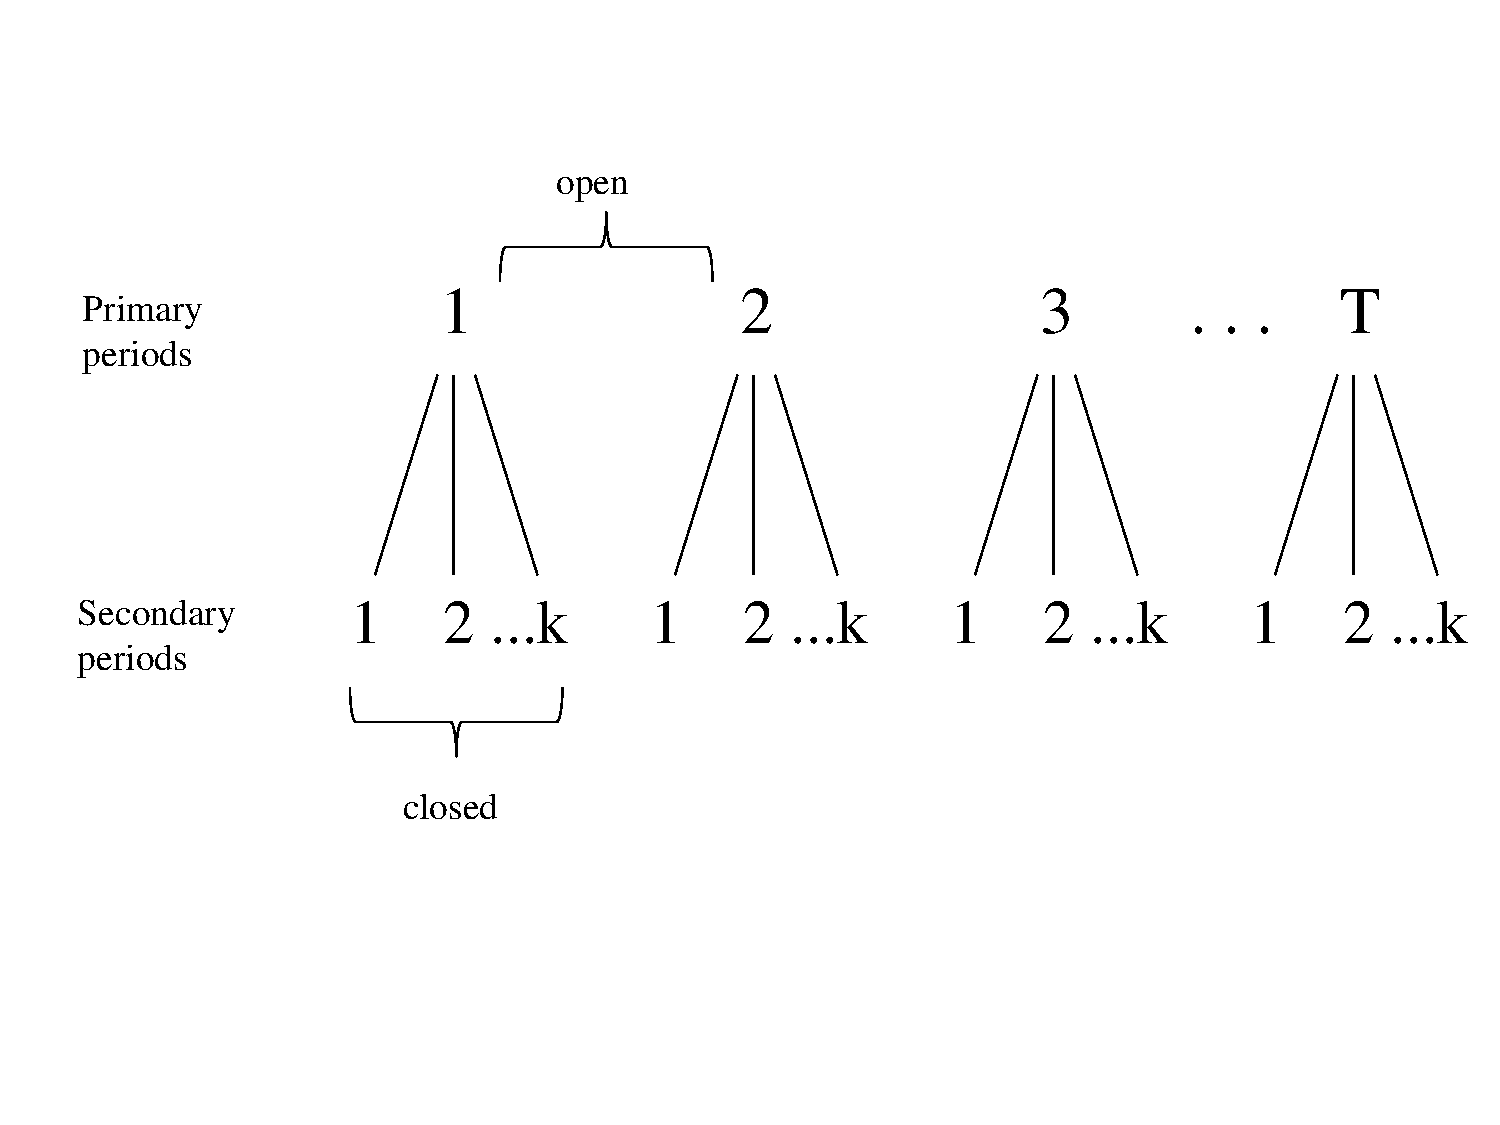
\includegraphics[height=2in,width=2.5in]{Ch16-Open/figs/RobustDesign.pdf}
\caption{Schematic of the robust design with T primary sampling periods and K secondary periods. The populations
are considered open between primary periods and closed within the secondary}
\label{open.figs.robustdesign}
\end{figure}

We can easily formulate
 a non-spatial JS
model using the robust design.  We 
define $y_{ikt}$ as the encounter history for individual
$i$ at secondary occasion $k$ during primary occasion $t$.  If we have
a Bernoulli encounter process then we can describe the observation
model, specified conditional on the ``alive state'', $z(i,t)$, for
individual $i$ at primary time $t$, as:
 \[
  y_{ikt}|z(i,t) \sim
\mbox{Bernoulli}(p z(i,t)).
\]
Thus, if individual $i$ is alive at time $t$ ($z(i,t)=1$), then the
observations are Bernoulli with detection probability $p$ as before.  Conversely, if the individual is
not alive ($z(i,t)=0$), then the observations must be fixed zeros with
probability 1. Note our distinct use of the variable $z$ here as
representing the state of individuals (alive/dead) instead of our
previous use of $z$ as the data augmentation variable. 

Survival and recruitment in the open population are manifest in a
model for the latent state variables $z(i,t)$ describing individual
mortality and recruitment events.  An important aspect of the
hierarchical formulation of the model that we adopt here is that the
model for the state variables is described conditional on the total
number of individuals ever alive during the study (a parameter which
we label $N$) based on $T$ periods, as in \cite{schwarz_arnason:1996}.  Data
augmentation induces a special interpretation on the latent state
variables $z(i,t)$.
In particular, ``not alive'' includes individuals
that have died, or individuals that have not yet been recruited.
\citep{royle_dorazio:2008} showed that using this formulation
simplifies the state model and also allows it
to be implemented directly in the \textbf{BUGS} language.
For example, considering the case $T=2$, the state model is composed
of the following two components: First the initial state is described
by:
\[
 z(i,1) \sim \mbox{Bernoulli}(\psi)
\]
and then a model describing the transition of individual states from
$t=1$ to $t=2$:
\[
 z(i,2) \sim \mbox{Bernoulli}( \phi z(i,1)  + \gamma (1-z(i,1)) ).
\]
If $z(i,1)=1$, then the individual may survive to time $t=2$ with
probability $\phi$ whereas, if $z(i,1)=0$, then the
``pseudo-individual'' may be recruited with probability $\gamma$.

We can then generalize this model for $T>2$ time periods and allow survival and
recruitment to be time dependent.  Initialize the
model for time $T=1$ as we have done above
and then the model describing the transition of individual states from
$t$ to $t+1$ is:
\[
 z(i,t+1) \sim \mbox{Bernoulli}( \phi_t z(i,t)  + \gamma_t (1-z(i,t)) ).
\]

This parameterization results in $T-1$ survival and recruitment
parameters.  The main difference here from the CJS model, described below,
 is that we include recruitment and are interested in estimating $N$ for each $t$.
Since this state model described above is conditional-on-$N$, we must
deal with the fact that $N$ is unknown, which is done through data
augmentation similar to how we used it in the closed population
models.


\subsection{Data augmentation for the Jolly-Seber model}

The fundamental challenge in carrying out a Bayesian analysis of this
model is that the parameter $N$ (the total number of individuals alive
during the study) is not known.  We have discussed and demonstrated
data augmentation in many previous chapters; however, with the open
population model, we have to take care that two issues are addressed:
(1) the data augmentation is large enough to accommodate all potential
individuals alive in the population during the entire study and (2)
that individuals cannot die and then re-enter the population.
\citep{royle_dorazio:2008} (see also \citet{kery_schaub:2011})  
describe this formulation for open
population models, including the non-spatial JS and robust design
models.

To begin, let's consider the role of recruitment, $\gamma$, in the
model when we use data augmentation to estimate $N$.
Data augmentation formally reparameterizes the model, replacing $N$,
the number of individuals ever alive with $M$, where we
assume $N \sim \mbox {Binomial}(M, \psi)$.  
%This is the same as having a discrete uniform prior on $N$, when the 
% prior for $\psi$ is $\mbox{Unif}(0,1)$.
That is, the expected value of $N$ under the model is equal to
$\psi M$.  As a result of this repararameterization, the recruitment
parameters $\gamma_{t}$ are also relative to the number of ``available
recruits'' on the data augmented list of size $M$, and not directly
related to the population size.  This can be dealt with
by deriving
$N_t$, and $R_{t}$, the population size and number of recruits in year
$t$, as a function of the latent state variables $z(i,t)$.  For
example, 
 the total number of individuals alive at time $t$ is
\[
N_{t} = \sum_{i=1}^{M} z(i,t)
\]
and the number of recruits is
\[
R_{t} = \sum_{i=1}^{M} (1-z(i,t-1))z(i,t)
\]
which is the number of individuals {\it not} alive at time $t-1$ but
alive at time $t$.

In the case of just two primary periods, this process is
straightforward.  When the number of primary sample occasions is
greater than 2, we must formulate the model for recruitment by
introducing another latent variable.  We do this in order to ensure
that an individual can only be recruited once into the population.
Here, this formulation of the model uses a set of latent indicator
variables, which we label $A(i,t)$,
which describe the time interval $(t-1, t)$ at
which individual is recruited into the population.  Let $A(i,t) = 1$
if individual $i$ is recruited in time interval $(t-1, t)$ otherwise
$A(i,t)=0$.  To construct the recruitment process we make use of the
standard conditional binomial construction of a removal process
(\citealt{royle_dorazio:2008}).  The initial state is given by:
\[
   A(i,1) \sim \mbox{Binomial}(1, \gamma_{1})
\]
for $i=1,2,\ldots,N$. Then, for $t>1$
\[
 A(i,t)|A(i, t-1) \dots A(i, 1) \sim \mbox{Binomial}((1 - \sum_{\tau=1}^{t-1} A(i, \tau) ) \times \gamma_{t}, 1)
\]
% XXXX What is tau here? XXXX  BETH:  it's just an index place holder, can't use t
Each recruitment variable is conditional on whether the individual was ever
previously recruited and this construction forces the recruitment
variable after initial recruitment to be degenerate (have a sample
size of 0).  Then, we can describe the state variables $z(i,t)$ by a
1st order Markov process.  For $t=1$, the initial states are fixed:
\[
z(i,1) \equiv A(i,1)
\]
and,
 for subsequent states, we have
\[
z(i,t)|z(i,t\,-\,1),A(i,t)
 \sim \mbox{Bernoulli} (\phi_{t} z(i,t\,-\,1)) \,+ \,  A(i,t).
\]
Thus, if an individual is in the population at time $t$ (i.e., $z(i,t)
= 1$), then that individual's status at time $t+1$ is the outcome of a
Bernoulli random variable with parameter (survival probability)
$\phi_{t}$.  If the individual, however, is not in the population at
time $t$ (i.e., $z(i,t) = 0$), then the outcome is a Bernoulli random
variable with probability $\gamma_{t}$, a parameter that is related to
{\it per capita} recruitment.  We carry out this process in \jags~ by
using the \mbox{\tt sum}() and \mbox{\tt step}() functions together to
ascertain if a particular individual $i$ was ever previously alive.
The \mbox{\tt step}() function is a logical test in \jags~ for $x \geq 0$
such that \mbox{\tt step}($x \geq 0$) returns a $1$, otherwise $0$.
Individuals that were ever previously alive are no longer eligible to
be ``recruited'' into the population.  The implementation of this model
in \jags~is shown in panel \ref{open.panel.nsJS}.


\begin{panel}[htp]
\centering
\rule[0.1in]{\textwidth}{.03in}
{\small
\begin{verbatim}
model{

psi ~ dunif(0,1)
phi ~ dunif(0,1)
p.mean ~ dunif(0,1)

for(t in 1:T){
N[t] <- sum(z[1:M,t])
gamma[t] ~ dunif(0,1)
 }

for(i in 1:M){
  z[i,1] ~ dbern(psi)	   #alive state for the first year
 cp[i,1] <- z[i,1]*p.mean
  Y[i,1] ~ dbinom(cp[i,1], K)     #the Y are the number of encounters
  a[i,1] <- (1-z[i,1])

for(t in 2:T){			   #for loop for years 2 to T
      a1[i,t] <- sum(z[i, 1:t])        #sum across the alive states from 1 to t
       A[i,t] <- 1-step(a1[i,t] - 1)   #A is the indicator if an individual
									   #is available to be recruited

       mu[i,t]<- (phi*z[i,t-1]) + (gamma[t]*A[i,t-1])
        z[i,t] ~ dbern(mu[i,t])        #alive state at t is dependent on phi and gamma
       cp[i,t] <- z[i,t]*p.mean
        Y[i,t] ~ dbinom(cp[i,t], K)
         }
         }
}
\end{verbatim}
}

\rule[-0.1in]{\textwidth}{.03in}
\caption{
\jags~model specification for the non-spatial JS model.}
\label{open.panel.nsJS}
\end{panel}



{\bf Mist-netting example}

We now return to the ovenbird data collected during a mist-netting
study, and initially presented in Chapt. \ref{chapt.poisson-mn}.  These data are available
in the \secr~package (see, \citet{efford_etal:2004,
  borchers_efford:2008}). To refresh your memory: 44 mist nets spaced
30 m apart on the perimeter of a 600-m x 100-m rectangle (see
Fig. \ref{open.figs.ovenbirdlocs}) were operated on 9 or 10 non-consecutive days in late May
and June for 5 years from 2005-2009.

\begin{figure}
\centering
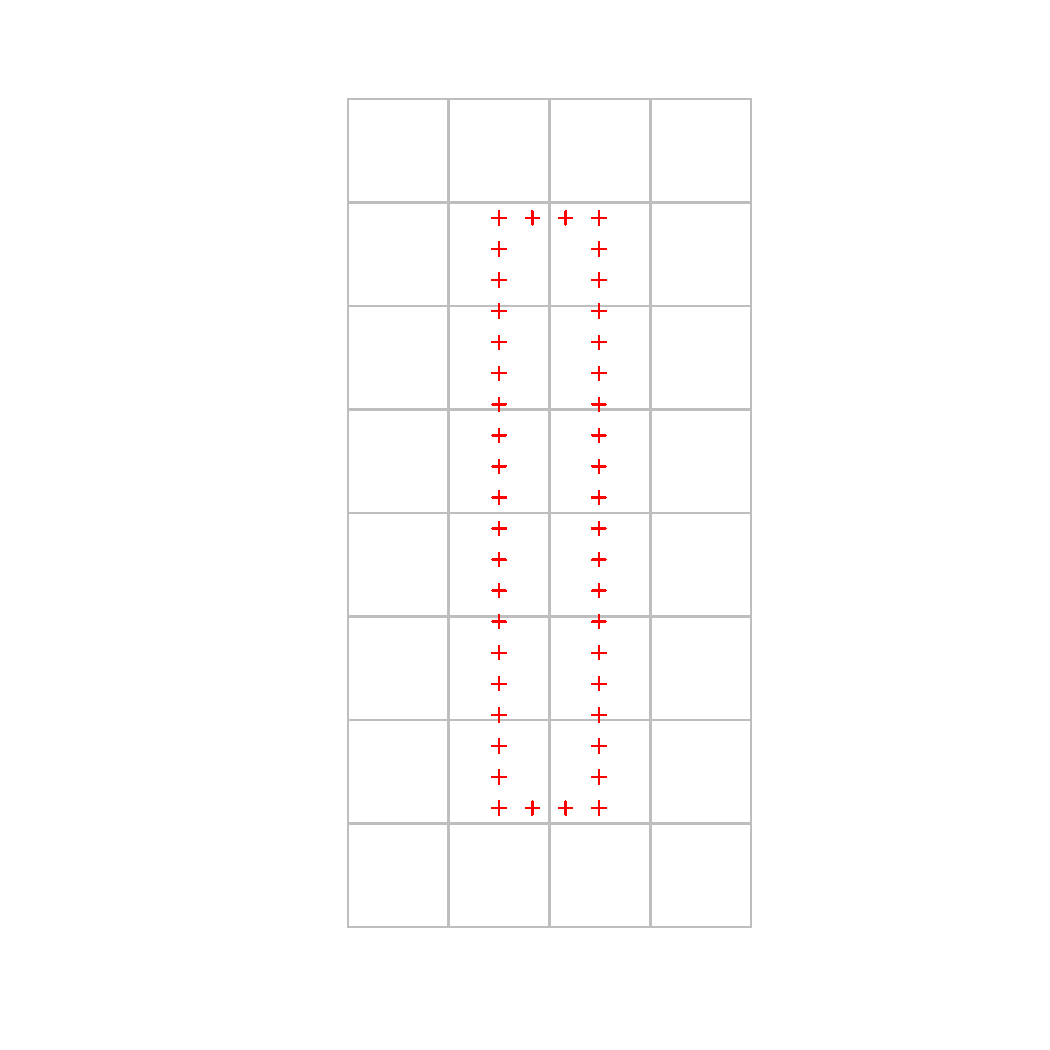
\includegraphics[height=2in,width=2.5in]{Ch16-Open/figs/ovenbirds.pdf}
\caption{Arrangement of the mist nests in the ovenbird study.  The nets are arranged in a 600-m by 100m
rectangle, spaced 30 m apart. }
\label{open.figs.ovenbirdlocs}
\end{figure}


In Chapt. \ref{chapt.poisson-mn}, we dealt with this dataset as a type
of ``multi-session''
model where abundance in each year, $N_{t}$, was estimated
separately. This
is the simplest approach for modeling data
collected over multiple years, but it does not allow for inference
about demographic processes, as does the JS model.


The first issue at hand is that each line in our 3-D encounter history
array of
data must correspond to a single individual.  Previously, we were not
interested in individual identity across years so this was not of
concern; however, we need to maintain the order of individuals across years
in order to estimate the survival and recruitment of the individual into the population.
We organize the data set so that each row in our
array represents just one individual across all primary periods.
For the ovenbird dataset, we
can organize the data by creating a master list of all individuals
captured during the entire study.  From this list, we can assign each
individual a unique row in our dataset (in the \R~ commands,
we do this by using the \mbox{\tt unique}() function
on the row names
for each year of our 3-D array and use \mbox{\tt pmatch}()
to associate the data to the correct column).  The code to carry out
this data organization are included in the \scrbook~ package and are not
shown here.  Additionally, in
Chapt. \ref{chapt.poisson-mn} we carried out data augmentation for each year separately;
however, we must consider for example that individuals captured in
year $t$ could have been alive in year $t-1$.  Our data
augmentation must be large enough to include individuals alive during
any of the time periods and to account for that, we set M=200.  For this example,
we hold survival constant but allow recruitment to be time dependent
(since $\gamma$ is essentially a function of the data augmentation
process as described above, it does not make sense to hold recruitment constant and we
therefore make it time specific).

To implement the model in Panel \ref{open.panel.nsJS}, the following commands
are used:

{\small
\begin{verbatim}
 #set initial values for the alive state, z
>zst<-c(rep(1,M/2),rep(0,M/2))
>zst<-cbind(zst,zst,zst,zst,zst)

>inits <- function(){list (z=zst,sigma=runif(1,25,100), gamma=runif(5,0,1)) }
>parameters <- c("psi","N","phi", "p.mean", "gamma")
>data <- list (K=10,Y=Ybin,M=M)

>library("rjags")
>out1 <- jags.model("modelNSJS.txt", data, inits, n.chains=3, n.adapt=500)
>out2NSJS <- coda.samples(out1,parameters,n.iter=20000)
\end{verbatim}
}

In this non-spatial JS model, N is estimated to be between about 22 and 33 for each of the 5 years (see
Table \ref{open.tab.JSmulti} for results).  The posterior mean for
detection (p.mean in the model) was 0.14, it
is not included in the table because the spatial models do not have
a parameter that directly corresponds to this one.  Instead, SCR models have a detection function
that is related to distance.


{\bf Shortcomings of the traditional JS models}

As we have previously discussed, one of the biggest shortcomings of the non-spatial
JS model is that we estimate $N$ but have no explicit spatial reference area for that
value.  As you see in Table \ref{open.tab.JSmulti}, the density estimate from the non-spatial JS model
is listed as NA.  This is because, again, the effective sampling area is unknown leaving us to
determine that area in an { \it ad hoc} manner.
Not making use of the
spatial information in the data makes
the estimation of density
a non-formal process.  As we saw in the closed models, the explicit
incorporation of spatial information will allow us to provide a robust estimate of density.
This improvement should
also carry through in our estimation of other demographic parameters
such as survival and recruitment as the movement of individuals is directly accounted for in the
model.


\subsection{Spatial Jolly-Seber models}

To parameterize the spatial JS models, we essentially follow all of the same steps
as the non-spatial model but we also include the trap location information into our
detection function.  Essentially, we are using the closed population SCR model to estimate
the detection parameters and initial population size,
and the open component is carried out in the process of how we model the transition
of $z(i,t)$ to $z(i, t+1)$ which is the same as in the non-spatial JS model.
To do so, we describe the Bernoulli observation model,
specified conditional on $z(i,t)$, as we have done throughout the book:

\[
  y_{ijkt}|z(i,t) \sim
\mbox{Bernoulli}(p_{ijk} z(i,t)).
\]
with
% \[
%\mbox{logit}(p_{ijk}) = \alpha_0 + \alpha_1 d_{ij}^2.
%\]
\begin{equation}
p_{ijk} = p_{0}*\exp(-\alpha_{1} d_{ij}^2)
\label{scr0.eq.norm}
\end{equation}
where $d_{ij}$ = $||{\bf s}_{i}-{\bf x}_{j}||$, the distance between
${\bf s}_{i}$ and ${\bf x}_{j}$.
% XXXX Remind the reader what p_0 and the alphas are

If individual $i$ is alive at time $t$ ($z(i,t)=1$), then the
observations are Bernoulli as before.  Conversely, if the individual is
not alive ($z(i,t)=0$), then the observations must be fixed zeros with
probability 1.  We can of course consider other encounter models such as the
Poisson or multinomial models described
in Chapt. \ref{chapt.poisson-mn}.

We initialize the
model for time $T=1$
and then model the transition of individual states from
$t$ to $t+1$ as:
\[
 z(i,t+1) \sim \mbox{Bern}( \phi_t z(i,t)  + \gamma_t (1-z(i,t)) ).
\]
Previously, we described how this formulation of the model uses a set of latent indicator
variables $A(i,t)$ which describes if individual is recruited into the population during time
$(t-1, t)$.  Therefore, $A(i,t) = 1$
if individual $i$ is recruited in time interval $(t-1, t)$ otherwise
$A(i,t)=0$.
Determining the number of recruits into the population,
%\[
%R_{t} = \sum_{i=1}^{M} (1-z(i,t-1))z(i,t),
%\]
%we can use a set of
can be done using two steps.
For example, to estimate the number of recruits from time period 1 to 2, we count those
individuals not in the population at time 1 ($z_{i,1} = 0$) but alive at time 2 ($z_{i,2} = 1$).
We can determine if individual $i$ has entered the population at time $t=2$ by using the formula:
 $R_{i,2}=(1-z_{i,1})z_{i,2}$ and then sum
$R_{i,2}$ over $M$ to get the total number of recruits.
We can do this for all the primary periods in our study,
as shown
in the \jags~code in Panel \ref{open.panel.spatialJS}.


\begin{panel}[htp]
\centering
\rule[0.1in]{\textwidth}{.03in}
{\small
\begin{verbatim}
model {

psi ~ dunif(0,1)    #set the priors
phi ~ dunif(0,1)
alpha0 ~ dnorm(0,10)
sigma ~dunif(0,200)
alpha1<- 1/(2*sigma*sigma)
A <- ((xlim[2]-xlim[1]))*((ylim[2]-ylim[1]))  #area

for(t in 1:T){
N[t] <- sum(z[1:M,t])   #calculate abundance for each year
D[t] <- N[t]/A			#calculate density for each year
R[t]<-sum(R[1:M,t])	    #calculate the recruits for each year
gamma[t] ~ dunif(0,1)   #prior for time specific recruitment parameter
}

for(i in 1:M){
  z[i,1] ~ dbern(psi)

  R[i,1]<- z[i,1]       #to estimate the number of recruits
  R[i,2]<-(1-z[i,1])*z[i,2]
  R[i,3]<- (1-z[i,1])*(1-z[i,2])*z[i,3]
  R[i,4] <-(1-z[i,1])*(1-z[i,2])*(1-z[i,3])*z[i,4]
  R[i,5] <-(1-z[i,1])*(1-z[i,2])*(1-z[i,3])*(1-z[i,4])*z[i,5]

  for(t in 1:T){
  S[i,1,t] ~ dunif(xlim[1],xlim[2]) # independent activity centers for each year
  S[i,2,t] ~ dunif(ylim[1],ylim[2])

  for(j in 1:ntraps){
    d[i,j,t] <- pow(pow(S[i,1,t]-X[j,1],2) + pow(S[i,2,t]-X[j,2],2),1)
     }
  for(k in 1:K){
    for(j in 1:ntraps){
      lp[i,k,j,t] <- exp(alpha0 - alpha1*d[i,j,t])*z[i,t]
      cp[i,k,j,t] <- lp[i,k,j,t]/(1+sum(lp[i,k,,t]))
    }
    cp[i,k,ntraps+1,t] <- 1-sum(cp[i,k,1:ntraps,t])  #last cell = not captured
    Ycat[i,k,t] ~ dcat(cp[i,k,,t])
  }
}
a[i,1]<-(1-z[i,1])
for(t in 2:T){                         #for loop for years 2 to T
      a1[i,t] <- sum(z[i, 1:t])        #sum across the alive states from 1 to t
       A[i,t] <- 1-step(a1[i,t] - 1)   #A is the indicator if an individual
									   #is available to be recruited at time t
       mu[i,t]<- (phi*z[i,t-1]) + (gamma[t]*A[i,t-1])
        z[i,t]~dbern(mu[i,t])
          }
        }
}
\end{verbatim}
}

\rule[-0.1in]{\textwidth}{.03in}
\caption{
\jags~model specification for the fully spatial JS model.}
\label{open.panel.spatialJS}
\end{panel}


{\bf Mist-netting example}

In the previous
analysis of the ovenbird data,
we did not make use of the spatial location for each net the ovenbirds were captured in.
However, there were 44 mist nets operational during
each of the sampling occasions.  We already organized the data above so that our 3-D encounter
histories are set up.  The data set is then $M=200$ individuals by $K=10$ secondary occasions
by $T=5$ primary occasions.  In the non-spatial version, we reduced the data to captured or
not-captured; however, the encounter history array, \mbox{\tt Yarr}, contains the number of the net that
each individual was captured in and contains a $45$ if the individual was not captured.  The
encounter history array, \mbox{\tt Yarr}), was created above in the code, so we do not
reproduce the code here. To call the model, use the following \R~ code which sets the initial
values for $z[i,t]$, the parameters to monitor, and calls \jags.


\begin{verbatim}

>zst<-c(rep(1,n),rep(0,M-n))
>zst<-cbind(zst,zst,zst,zst,zst)

>inits<-function(){list(z=zst,sigma=runif(1,25,100),
              gamma=runif(5,0,1), S=Sst,alpha0=runif(1,-2,-1))}
>parameters<-c("psi", "alpha0", "alpha1", "sigma", "N",
                       "D", "phi", "gamma", "R")
>data <-list(X=as.matrix(X[[1]]), K=10, Ycat=Yarr,
              M=M, ntraps=ntraps, ylim=ylim, xlim=xlim)
>library("rjags")
>out1<-jags.model("modelJS.txt", data, inits, n.chains=3,
             n.adapt=500)
>out2JS<-coda.samples(out1,parameters,n.iter=10000)

\end{verbatim}



\begin{table}
\centering
\caption{
Posterior mean of model parameters for the non-spatial JS model (NS-JS), the spatial JS model (S-JS),
and the spatial multi-season model (S-MS) fitted to the
ovenbird data set.  Density shown in individuals per hectare.
}

\begin{tabular}{crrr}
\hline \hline
    &   NS-JS &   S-JS   &   S-MS \\  \hline
D[1]    &  NA & 0.96 &  0.93   \\
D[2]     & NA & 1.00 &  1.00  \\
D[3]   &   NA & 1.10 &  1.20  \\
D[4]   &   NA & 1.10 &  0.89 \\
D[5]   &   NA & 0.79  & 0.76  \\
N[1]   &  26.5 &  33 &  32.4  \\
N[2]   &  30.2 &  36 &  35.8  \\
N[3]    & 33.1 &  39 &  42.1 \\
N[4]   &  29.5 &  37 &  30.8 \\
N[5]   &   21.7 & 28 &  26.2 \\
alpha0 &   NA & -2.9 & -2.88  \\
alpha1  &   NA & 1.2e-04 & 1.22e-04  \\
sigma  &   NA &  6.4 & 6.44 \\
gamma[1]  & 0.50 &  0.50 & NA \\
gamma[2] &  0.09  & 0.09 & NA \\
gamma[3] &  0.11 & 0.13 & NA \\
gamma[4] &  0.13 & 0.16 & NA \\
gamma[5] &  0.07 & 0.08 & NA \\
phi   &  0.48 &   0.53 & NA \\
psi   &  0.14 &  0.17 & NA \\
R2    &  NA &   15 & NA \\
R3    &   NA &   19 & NA \\
R4    &   NA &   8.3 & NA \\  % XXXX How can this be a fraction?  BETH: It's the mean over all iterations.
R5    &   NA &   8.3 & NA \\ \hline
\end{tabular}
\label{open.tab.JSmulti}
\end{table}

Our results for density, alpha0, and alpha1 are rather similar to those found in the multi-season
analysis from Chapt. \ref{chapt.poisson-mn}.
Since all of our parameters including alpha0 and alpha1 are shared between seasons, we
would expect these results to be similar between the multi-season model and the JS model (see Table \ref{open.tab.JSmulti}).
There are some slight differences in the parameter estimates, for example, the density is smaller
in year 4 in the multi-season model than in the JS model.  This maybe be due to a smaller sample size in that year and the JS model is able to
make use of the data a little more efficiently across the years.   Because we have defined the same state space for
the spatial JS model and multi-season, our estimates of $N$ are directly comparable.  However, the estimates of $N$
under the  non-spatial JS model are not directly comparable as we do not have a well-defined effective trapping area.
We see from Table \ref{open.tab.JSmulti} that $N$ is smallest for the non-spatial JS model across all years.
This suggests that the actual effective trapping area is smaller than our state space, but we cannot know how much relative to the state space to make useful comparisons between the $N$s.


\begin{figure}
\centering
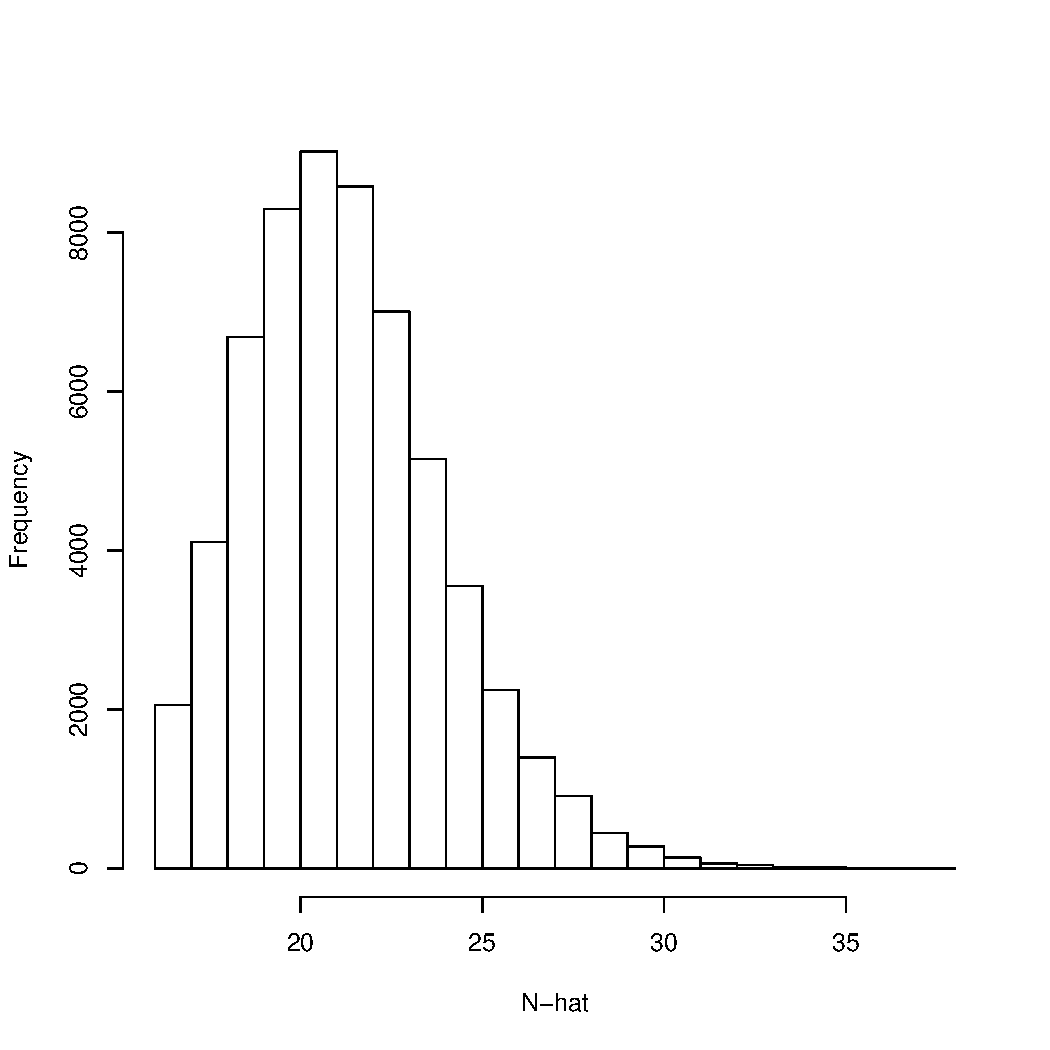
\includegraphics[height=2in,width=2.5in]{Ch16-Open/figs/Nhat5ovenbird.pdf}
\caption{Posterior distribution of $N_5$ from the spatial JS model for the ovenbird dataset.  This graph suggests that there is no truncation of the posterior of $N_5$. }
\label{open.figs.ovenbirdN5hist}
\end{figure}

% XXXX Great practical advice here XXX
In the JS formulation of the model, we also estimate the recruitment for each year,
and we can look at our derived values for recruitment (R2, R3, R4, and R5).
R2 is the number of new
recruits from primary period 1 to 2; R3 is the number of new recruits from primary period 2 to 3; and so forth.
R2 and R3 are almost
double that of R4 and R5, suggesting that less animals were recruited into the population in the latter years
of the study.  The density in
the last year of the study was lower than previous years.
It is good to check your results when you see a pattern like this -- the number
of recruits declining each year -- because this could be an indication that the data augmentation was not large enough.
In this example,
we checked to make sure that M=200 was sufficiently large by examining the recruitment parameter,
$\gamma$.  If $\gamma$ is close to 1 during any of the time periods, then there are not enough
augmented individuals in the overall dataset.  In this case, the 97.5\% quantile of $\gamma_5$,
the recruitment probability in the final year of the study, was 0.14 and none of the other $\gamma$s
 were close to 1 either.  You can also look at the posterior distributions of $N$ to make sure
they are not truncated, Fig. \ref{open.figs.ovenbirdN5hist} shows that the posterior distribution of $N_5$ is not
truncated. The posterior mean for survival, $\phi$, was 0.53.  Although we did not do it here,
it should be easy to see that we could allow survival to vary by time, as we did with recruitment.
Our estimates of survival seem
reasonable when compared with the literature.  Some studies have found annual male ovenbird
survival to be around 0.62 \citep{porneluzi_faaborg:1999, bayne_hobson:2002}; however,
female ovenbird
survival was much lower (0.21,
\cite{bayne_hobson:2002}). With more individuals, we could run this model with survival
estimated for each sex separately.
However, researchers should be careful not to over-parameterize models based on the amount of
data available.   The results indicate that the posterior mean estimate of $\phi$ was greater in the SCR
model (0.53) than the non-spatial model (0.48) which suggests that the SCR model is starting to separate
movement from survival in order to estimate the true survival.



\section{Cormack-Jolly-Seber models}

\subsection{Traditional CJS models}

The Cormack-Jolly-Seber models are used extensively in the literature
to estimate survival probabilities.  There are essentially two ways to
fit these models, using either a
multinomial approach \citep{lebreton_etal:1992} or a state space
likelihood approach \citep{gimenez:2007, royle:2008}.
% XXXX Can you compare/contrast them?

We can adopt a simple hierarchical parameterization of the
basic single state, non-spatial CJS model in which the observation model is
described conditional on the latent state variables $z(i,t)$ -- the
``alive state" which describe whether individual $i$ is
alive ($z(i,t)=1$) or not ($z(i,t)=0$) during each of $t=1,2,\ldots,T$
{\it primary} periods.
% XXXX Explain if this is the multinomial or state space appraoch
Let $y_{it}$ indicate the observed
encounter data of individual $i$ in primary period $t$. The
model, specified conditional on $z(i,t)$, is:
 \[
  y_{it}|z_{it} \sim
\mbox{Bernoulli}(p_{t}z_{it}).
\]

Analogous to the JS model, if individual $i$ is alive at time $t$ ($z_{it}=1$),
then the observations are Bernoulli with probability of detection $p_t$.
If the
individual is not alive ($z_{it}=0$), then the observations must be
fixed zeros with probability 1.
In the CJS formulation, as opposed to the JS, we condition on first capture which means that $z_{it}$ will
be 1 when $t$ is the first primary period of capture.   We can denote this $z_{i f_i}$
where $f_i$ indicates the primary occasion in which individual $i$ is first captured, which
can vary from $1 \dots T$.
This ensures that each individual is alive upon entering the model.

The ''alive state" at time $t$ for each individual is a
function of the state at the previous time step $t-1$.   Because
we condition on the first capture, the initial
state is set to one:
\[
 z_{i f_i} = 1
\]
where $f_i$ indicates the primary occasion in which individual $i$ is
captured and the model for the transition of individual states from $t$ to $t+1$ for
all $t > f_i$ is
\[
 z_{i t} \sim \mbox{Bernoulli}( \phi z_{i,t-1}).
\]
Because we start with $z_{i f_i} = 1$, the individual survives with probability
$\phi$ to time $f_i + 1$ and so forth.  Once an individual leaves the
population (i.e., $z_{it} = 0$), there is no mechanism for the
individual to return.
This means that under this specification individuals cannot
temporarily emigrate.  In the CJS model we are not estimating $N$, so we do not incorporate
any data augmentation here.  This version of the model is easy to construct in the \bugs~ (or \jags)
language which is shown in Panel \ref{open.panel.nsCJS}.  Variations on this basic model and associated code for
fitting the model in \bugs~ are described in detail in \citet[][Chapts. 7-9]{kery_schaub:2011}.

\begin{panel}[htp]
\centering
\rule[0.1in]{\textwidth}{.03in}
%\begin{minipage}{2.5in}
{\small
\begin{verbatim}
model{
phi ~ dunif(0,1)   #Survival (constant over time)

for(t in 1:T){
p[t] ~ dunif(0, 1)    #detection (varies with time)
}

for (i in 1:M){
   z[i,first[i]] ~ dbern(1)
  for (t in (first[i]+1):T) {
         tmp[i,t] <- z[i,t]*p[t]
           y[i,t] ~ dbern(tmp[i,t])
       phiUP[i,t] <- z[i,t-1]*phi
           z[i,t] ~ dbern(phiUP[i,t])
   }
  }
 }
\end{verbatim}
}

\rule[-0.1in]{\textwidth}{.03in}
\caption{
\jags~ model specification for the non-spatial basic CJS model.}
\label{open.panel.nsCJS}
\end{panel}


\begin{figure}
\centering
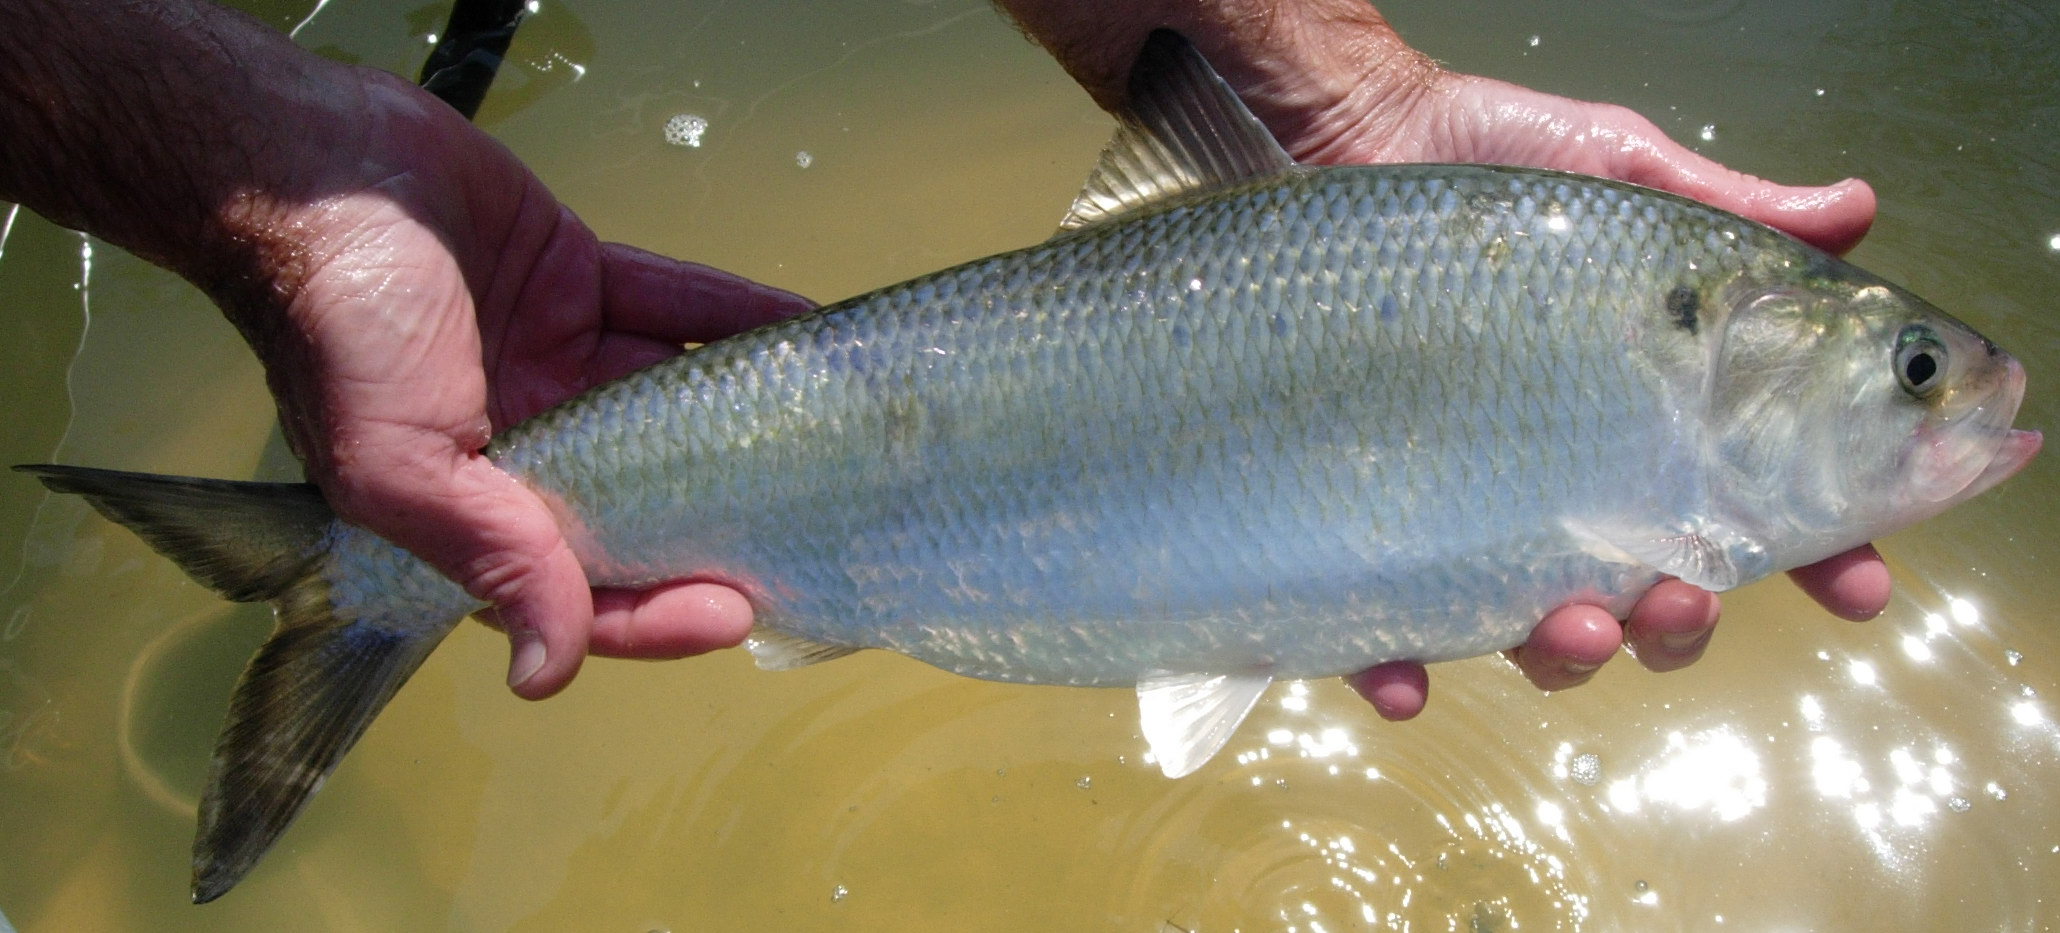
\includegraphics[height=2in,width=4.43in]{Ch16-Open/figs/American_Shad_Raabe.jpg}
\caption{American shad caught in North Carolina, U.S.A.  Credit: Joshua Raabe, North Carolina State University}
\label{open.figs.shadpic}
\end{figure}

{\bf Migratory fish example}
The motivation for this example stems from an interest in better
understanding survival and movement of migratory fishes.  For this
example, we will use data collected on American shad \textit{Alosa sapidissima}
in the New River in North Carolina, U.S.A. (see photo in Fig. \ref{open.figs.shadpic}).
The data were collected and analyzed in \cite{raabe_diss:2012}.
Using a resistance board weir near the
river mouth, 315 fish
were tagged with passive integrated transponders (PIT) in the spring
of 2010. An array of 7 upstream PIT antennas passively recaptured
individuals during upstream and downstream migrations.  Each time a fish passed
over the antenna, it was recorded and summarized weekly for 12 weeks. The
fish do not necessarily move past all antenna and may remain in the river between
antenna for more than a week, thus they are not all detected at each time period.
The antenna do not always operate perfectly either and fish that pass may not be recorded
at some times.

To apply the basic CJS model, we create the
encounter history for each individual for the 12 weeks and we also create
a vector to indicate the period of first capture.
% XXXX Do you have a map of the river with the receiver locations?

\begin{table}
\centering
\caption{Results of the basic non-spatial CJS model for the American shad dataset.
}
\begin{tabular}{crrrrr}
\hline \hline
&    Mean   &  SD  &  2.5 \%   &   50 \%    &  97.5 \% \\
p[1] & 0.499 & 0.289 & 0.026 & 0.499 & 0.975 \\
p[2] & 0.627 & 0.058 & 0.511 & 0.628 & 0.738 \\
p[3] & 0.762 & 0.036 & 0.689 & 0.763 & 0.829 \\
p[4] & 0.880 & 0.025 & 0.828 & 0.882 & 0.925 \\
p[5] & 0.548 & 0.043 & 0.465 & 0.548 & 0.633 \\
p[6] & 0.259 & 0.038 & 0.190 & 0.258 & 0.337 \\
p[7] & 0.126 & 0.031 & 0.072 & 0.124 & 0.194 \\
p[8] & 0.236 & 0.045 & 0.155 & 0.234 & 0.332 \\
p[9] & 0.237 & 0.049 & 0.148 & 0.234 & 0.341 \\
p[10]& 0.589 & 0.072 & 0.447 & 0.590 & 0.728  \\
p[11]& 0.834 & 0.063 & 0.700 & 0.839 & 0.942 \\
p[12]& 0.468 & 0.072 & 0.330 & 0.466 & 0.614 \\
$\phi$  & 0.824 & 0.011 & 0.802 & 0.825 & 0.846 \\
\hline
\end{tabular}
\label{open.tab.simple-shad}
\end{table}

Table \ref{open.tab.simple-shad} shows the estimated detection probability for each of the 12 primary periods
in the study.  The posterior mean for detection probability ranges from 0.126 to 0.880, which could potentially
be due to variation in water flow, stream depth, storms, etc$\dots$  The weekly survival probability, $\phi$ had a
posterior mean estimate of 0.824.  This estimate could be considered low for a weekly probability, but
is likely due to the fact
that the migration upstream can be quite energetically taxing and the fish are likely to only feed minimally
in rivers(\citep{leggett_carscadden:1978, leonard_mccormick:1999}).
Additionally, the CJS model is only estimating apparent survival
and some fish may have left the stream temporally or permanently heading back to the ocean
or possibly to other tributaries that are not monitored.
We demonstrate in panel \ref{open.panel.nsCJS}
how to allow $p$ to vary by time, but we could also allow survival, $\phi$ to vary by time by
implementing it exactly as
we do $p$.
As we move into the multi-state model,
we can test for movement and survival by state, which allows more specific biological questions to be addressed.



\subsection{Multi-state CJS models}

The basic version of the CJS model only allows for estimation of survival and detection.  However,
researchers are often interested in addressing other ecological questions such as age-dependent
survival rates, habitat based movements, etc.  Multi-state models allow researchers to directly
address such questions by incorporating more than one state that an individual may potentially
be in \cite{arnason:1972,arnason:1973, brownie_etal:1993}.  These possible states can be geographic
location, age class, or reproductive status among many
others.  Instead of just having an encounter history for an individual, we will also have auxiliary
information on the state of that individual at capture (e.g., breeder or non-breeder).
Since our interest is in movement of individuals, here we will consider states that represent spatial units or
geographic locations.  Generally speaking, we might think that the transition rates between locations could be due to
habitat features (or quality) and we can use multi-state models to help us address such a question.
In addressing movement through a multi-state modeling approach, the movement is often parameterized
as random or Markovian between patches (\cite{arnason:1972,arnason:1973, schwarz_etal:1993}).

In the simplest version of the multi-state model we have just two states.  Thus, individuals
can be marked and recaptured in one of two states (we'll call them A and B here).
We will assume that the two ``states'' are different
geographic sites.
In our single-state model above, an individual $i$ was either alive ($z_{it}=1$) at time $t$
or dead ($z_{it}=0$).  Now, we must consider that the individual could be alive in a given state or
dead and that individuals can transition between states.  An easy way to think about this is to look at
the state transition matrix in Table \ref{open.tab.CJSmulti-matrix}.
Here, $\phi_A$ % XXXX suggest using superscript A and B to avoid
               % confusion with subscripts
is the probability of surviving
in State A from time $t$ to $t+1$ and $\phi_B$ is analogous for State B.  The
movement parameters are $\psi_AB$ and $\psi_BA$,
where $\psi_AB$ is the probability that an individual, which survived
from $t$ to $t+1$ in Site A, moves to State B just
before $t+1$ and vice versa for $\psi_BA$


\begin{table}[htb!]
\centering
\caption{
Transition matrix for a multi-state model with just two states.
}
\begin{tabular}{crrr}
\hline \hline
    &   State A &   State B   &   Dead \\  \hline
State A & $\phi_A(1-\psi_{AB})$ & $\phi_A \psi_{AB}$ & 1 - $\phi_A$ \\
State B & $\phi_B \psi_{BA}$ & $\phi_B(1-\psi_{BA})$ & 1 - $\phi_B$ \\
Dead & 0 & 0 & 1\\ \hline
\end{tabular}
\label{open.tab.CJSmulti-matrix}
\end{table}

We do not necessarily observe individuals in their given state though, so we must estimate detection
separately for each of the states.  Hence we also have $p_A$ and $p_B$, the probability of detecting
an individual in state A and state B respectively.

To relate this back to the description of multi-state models in Chapt. \ref{chapt.poisson-mn}, we can define ${\bf s}$
as the index of which state an individual is in and $u_{it}$ as
the state in which individual $i$ was observed during sample $t$.  In this two state example,
$u_{it}$ can only take on values for being observed in A or B (i.e., 1 or 2).

We can define a simplistic model such that
\[
u_{it} \sim  \mathrm{dcat}(\psi)
\]
where $\psi$ is a constant vector.
We observe that individual with probability $p_{0}$, that is:
\[
 \Pr(y_{it} = 1| u_{it} )  = p_{0}
\]
The state-transition probabilities are constant.


To extend this model, we can define ${\bf s}$
as the index of which state
an individual is in and then condition the observed locations, $u_{it}$
as a function of the state an individual is in, ${\bf s}$. This
means that whether an individual moves or not, or where it moves to, is a function of where it is located.

This commonly used model has successive movement outcomes that
are $iid$
\[
u_{it} \sim  \text{dcat}( {\psi}({\bf s}_{i}) )
\]

Conditional on the state in which individual $i$ is located, we
observe that individual with probability $p_{0}$. That is:
% XXXX This is same as second-to-last equation
\[
 \Pr(y_{it} = 1| u_{it} )  = p_{0}
\]
The state-transition
probabilities are still constant, conditional on ${\bf s}$.
Other models for these transition probabilities
are possible and we will discuss those later.

A slight modification of this model would define ${\bf s}$  as a
``home area'' % XXXX or home range?
 for each individual. Then
the region the animal goes to is a function, not of where he was last time, but which region is his home area.
This model is only subtlety different from the Markovian model and as was shown in Chapt. \ref{chapt.poisson-mn}
for closed populations models is how we make the technical transition from multi-state models to SCR models.
Essentially increasing to a large number of strata, this formulation of the multi-state model becomes an SCR model
where the ``area of activity'' ${\bf s}$ becomes the ``activity center" for
each individual.

To program this model in \jags, we use a slightly different formulation which essentially combines
$u_{it}$ and $y_{it}$ as defined above into one observation matrix such that $y_{it} = 1, 2,$ or $3$ where
3 indicates ``not observed''.  Additionally, we use $z_{it}$ to indicate the true state of individual
$i$ such that $z_{it} = 1, 2,$ or $3$ where 1 indicates alive and in state 1, 2 indicates alive and in state 2,
and 3 indicates ``not alive''.  Using this delineation, we just need to set up the transition
matrix based on Table \ref{open.tab.CJSmulti-matrix}
and define each item within the model specification, shown in Panel \ref{open.panel.msCJS}.
Note that this can become quite cumbersome when dealing with models that
have many states.


\begin{panel}[htp]
\centering
\rule[0.1in]{\textwidth}{.03in}
%\begin{minipage}{2.5in}
{\small
\begin{verbatim}
model{
for(r in 1:2){
phi[r] ~ dunif(0,1)
psi[r] ~ dunif(0,1)
p[r] ~ dunif(0,1)
}

for (i in 1:M){
    z[i,first[i]] <- y[i, first[i]]
for (t in (first[i]+1):T){
    z[i,t] ~ dcat(ps[z[i,t-1], i, ])
    y[i,t] ~ dcat(po[z[i,t], i, ])
}
	ps[1, i, 1] <- phi[1] * (1-psi[1])
	ps[1, i, 2] <- phi[1] * psi[1]
	ps[1, i, 3] <- 1-phi[1]
	ps[2, i, 1] <- phi[2] * (1-psi[2])
	ps[2, i, 2] <- phi[2] * psi[2]
	ps[2, i, 3] <- 1-phi[2]
	ps[3, i, 1] <- 0
	ps[3, i, 2] <- 0
	ps[3, i, 3] <- 1

	po[1, i, 1] <- p[1]
	po[1, i, 2] <- 0
	po[1, i, 3] <- 1-p[1]
	po[2, i, 1] <- 0
	po[2, i, 2] <- p[2]
	po[2, i, 3] <- 1-p[2]
	po[3, i, 1] <- 0
	po[3, i, 2] <- 0
	po[3, i, 3] <- 1
}
}
\end{verbatim}
}

\rule[-0.1in]{\textwidth}{.03in}
\caption{
\jags~ model specification for a two state version of the multi-state CJS model. Code adjusted
from \cite[][Chapt. 9]{kery_schaub:2011}. }
\label{open.panel.msCJS}
\end{panel}


{\bf Migratory fish example}

Previously, we analyzed the American shad data using a basic CJS
model.  However,
the researchers were interested in movement of fish during migration and so we
classified the stream into 2 states (regions) -- ``downstream" and ``upstream".  Each antenna was assigned
to a state based on the location, those below 20 river kilometers were considered in
the downstream state.  Each fish has an encounter history including whether or not the fish was
detected during each week of the 12 week study, but also the ``state'' of capture
(``downstream'' or ``upstream'').  Again, a vector to indicate the period of first capture was also
created.  Fish captured in more than one state during the week were assigned the state in which
they were captured most during that week.


\begin{table}
\centering
\caption{
Results of the multi-state CJS model for the migratory fish example.  $p_A$ is the detection probability in the first state (A), which in this case is the down stream area.  $phi_A$ is the weekly survival probability in state A and $\psi_AB$ is the probability that an individual, which survived from $t$ to $t+1$ in Site A, moves to State B just
before $t+1$.
}
\begin{tabular}{crrrrr}
\hline \hline
&       Mean   &  SD  &  2.5 \%   &   50 \%    &  97.5 \%  \\  \hline
$p_A$ & 0.777 & 0.045 & 0.689  & 0.777  & 0.866 \\
$p_B$  & 0.434  & 0.027 & 0.382 & 0.434  & 0.489 \\
$\phi_A$  & 0.850 & 0.022 & 0.807  & 0.851  & 0.893  \\
$\phi_B$  & 0.782  & 0.019 & 0.743  & 0.782& 0.820  \\
$\psi_AB$ & 0.421 & 0.034 & 0.356  & 0.421 &  0.489 \\
$\psi_BA$& 0.927 & 0.014 & 0.897  & 0.937 &  0.952  \\

\hline
\end{tabular}
\label{open.tab.multi-shad}
\end{table}

Survival between the two areas is quite different (see Table \ref{open.tab.multi-shad}).  This might suggest that
fish moving further upstream are expending more energy and are more likely to die.
While survival in the two states was different, it is intuitive that the average of the survival
probabilities for A and B is essentially the same as that from the
basic non-spatial CJS ($\phi = 0.82$, see Table
\ref{open.tab.simple-shad}).   Also, it should be noted
that $\psi_BA$ is very high, indicating that fish in this study are
returning downstream after spawning in the upstream area.
These results highlight the utility in using a multi-state model to understand movement between states; here,
we used spatial states, but age, class, breeding status, etc. are all possibilities.  We did have to reduce the
<<<<<<< HEAD
dataset however to fit this model and information on spatial location was lost in creating just two states, downstream and upstream.  Losing information is one potential effect of using a multi-state model, additionally when states are hidden or unknown (e.g., when animals are in a region not exposed to
sampling), these models can be difficult to fit (XXX cite Sarah?).  Both of these issues can be resolved using the fully spatial
CJS model.
=======
dataset however to fit this model and information on spatial location was lost in creating just two states, downstream and upstream.  Losing information is one potential effect of using a multi-state model, additionally when states are hidden or unknown (e.g., when animals are in a region not exposed to 
sampling or the state is misclassified), these models can be difficult to fit (see \citep{conn_cooch:2009} for an overview of these problems).   Not losing information and unknown states are two issues that can be resolved using the fully spatial CJS model.   Misclassification of state (or even individual) is a difficult problem to solve and current approaches (\cite{link_etal:2010, mcclintock_etal:inpress}). 
>>>>>>> final edits


\subsection{Spatial CJS models}

In Chapt. \ref{chapt.poisson-mn}, we described how SCR models are
essentially a type of multi-state model with spatially structured transition probabilities.
As we noted, individuals can appear in $>1$ states, simultaneously,
which is not directly analogous to a standard multi-state model.  However, building on the state space and
multi-state CJS models, we can
explicitly incorporate individual movement as an
individual covariate model \citep{royle_indcov:2007}.
To move from the basic and multi-state CJS models to the SCR version, we need only make a few
changes to the model.  Essentially, we will not have discrete states and thus the biggest
difference is that individuals do not ``transition'' between a finite set of states, but
instead are allowed to move in continuous space.

We may consider the same basic encounter
models as described previously (i.e., Poisson, Bernoulli, or
multinomial). In particular, let $y_{ijkt}$ indicate the observed
encounter data of individual $i$ in trap $j$, during interval
(secondary period or sub-sample) $k=1,2,\ldots,K$ and primary period $t$. We note that in
some cases we may have intervals ($K=1$) which correspond to the
design underlying a standard CJS or JS models whereas the case $K>1$
corresponds to the ``robust design'' (\citealt{pollock:1982}).  The
Poisson observation model, specified conditional on $z(i,t)$, is:
 \[
  y_{ijkt}|z(i,t) \sim
\mbox{Poisson}(\lambda_0 g_{ij} z(i,t)).
\]
% XXXX Remind people what g is
%If individual $i$ is alive at time $t$ ($z(i,t)=1$), then the observations are Poisson as before.
Conversely, if the
individual is not alive ($z(i,t)=0$), then the observations must be
fixed zeros with probability 1.   In the CJS formulation, we will condition on first capture
which means that $z(i,t)$ will
be 1 when $t$ is the first primary period of capture.  We can denote this $z(i, f_i)$
where $f_i$ indicates the primary occasion in which individual $i$ is first captured.
This ensures that each individual is alive upon entering the model.

Modeling time-effects either
within or across primary periods
is straightforward. For that, we define $\lambda_{0} \equiv
\lambda_{0}(k,t)$ and then develop models for
$\lambda_{0}(k,t)$ as in our closed SCR models (we note that
trap-specific effects could be modeled analogously).


We follow the same model for survival as described in the non-spatial version of the
CJS.  The model is initialized by setting the alive
state at first capture to one:
\[
 z(i,f_i) = 1
\]
and for the transition of an individual's alive state from $t$ to $t+1$, for
all $t > f_i$, we have
\[
z_{it} \sim \mbox{Bernoulli}( \phi z_{i,t-1}).
\]
An individual survives with probability
$\phi$ from one time step to the next.  It is easy to see that we can let
survival be time specific by allowing $\phi$ to vary with each time step:
\[
 z_{it} \sim \mbox{Bernoulli}( \phi_t z_{i,t-1}).
\]

In either case, once an individual leaves the
population (i.e., $z_{it} = 0$), there is no recruitment so individuals cannot
return.  Again, we are not estimating $N$ in this model, hence we do not need
any data augmentation.  This conveniently makes the model run
faster too!



{\bf Migratory fish example}

Going back to our American shad example, we can consider that this is
exactly a spatial capture recapture problem.
In stream networks, the placement of PIT antennas along the stream mimics the
type of spatial data collected in terrestrial passive detector arrays such as
camera traps, hair snares, acoustic recording devices, etc.  The
difference is that for fish and aquatic species, the stream constrains
the movement of individuals to a linear network.  Using the data from the
array of 7 PIT antennas and the number of
times each fish passed over the antenna, we can apply the SCR CJS model to
evaluate movement up and downstream of these fishes.
When we look at the individuals encountered at each antenna for each of the primary periods,
the dimensions of the data are 315
individuals by 7 antennas by 12 sample occasions. Individuals can
encounter any antenna any number of times during the week, which means
we just sum the encounters over the week and eliminate any need for
explicit secondary occasions in the model. The result is a 3-D array
instead of a 4-D array.  Given the structure of the encounters, we use
a Poisson encounter model in this example.

% XXXX Suggest sticking with your format of putting BUGS code in a
% panel, and keeping R code seperate. And add more comments. XXXX
{\small
\begin{verbatim}
library(reshape)

# Constants:
M <- 315       # Number of individuals
T <- 12        # Number of periods (weeks)
nantenna <- 7  # weir, 6 antennas
antenna.loc <- c(3,7,12,44,56,72,77)  # antenna locations

# Input and format data matrix:
AS10 <- read.table("AS10.txt" ,header=T)
melted.rkm <- melt(AS10, id=c("TagID","RKM"))
y <- cast(melted.rkm, TagID ~ RKM ~ value, fill=0, length)
first=read.csv("firstcap.csv")

sink("ModelCJS.txt")
cat("

model {
# Priors
sigma ~ dunif(0,80)
sigma2 <- sigma*sigma
lam0 ~ dgamma(0.1, 0.1)
phi ~ dunif(0, 1)   # Survival (constant across time)
tauv~dunif(0, 30)
tau<-1/(tauv*tauv)

for (i in 1:M){
  z[i,first[i]] <- 1
  S[i,first[i]] ~ dunif(0,50)

for(j in 1:nantenna) {
	  D2[i,j,first[i]] <- pow(S[i,first[i]]-antenna.loc[j], 2)
       lam[i,j,first[i]]<-  lam0*exp(- D2[i,j,first[i]]/(2*sigma2))
       tmp[i,j,first[i]] <- lam[i,j,first[i]]
         y[i,j,first[i]] ~ dpois(tmp[i,j,first[i]])
      }

   for (t in first[i]+1:T) {
	          S[i,t] ~ dunif(xl, xu) # XXXX above you have dunif(0,50)?
         for(j in 1:nantenna) {
		        D2[i,j,t] <- pow(S[i,t]-antenna.loc[j], 2)
               lam[i,j,t] <- lam0 * exp(-D2[i,j,t]/(2*sigma2))
	           tmp[i,j,t] <- z[i,t]*lam[i,j,t]
		         y[i,j,t] ~ dpois(tmp[i,j,t])
		 }
 	   phiUP[i,t] <-  z[i,t-1]*phi
	       z[i,t] ~ dbern(phiUP[i,t])
	}
	}
}

",fill = TRUE)
sink()

data1<-list(y=y, first=first, M=M, T=T, xl=0, xu=80, nantenna=nantenna, antenna.loc=antenna.loc)

z=matrix(NA, M, T)
for(i in 1:M){
for(t in first[i]:12){
z[i,t] <-1
}
}

inits =  function() {list(z=z,phi=runif(1,0,1), lam0=runif(1,0,2),
                     tauv=runif(1,10, 20), sigma=runif(1,0,10)) }

parameters <- c("sigma", "phi", "lam0")

library("rjags")
out1 <- jags.model("modelCJS.txt", data1, inits, n.chains=3, n.adapt=500)
out2CJS <- coda.samples(out1,parameters,n.iter=20000)
\end{verbatim}
}

\begin{table}
\centering
\caption{
Results of the spatial CJS model fitted to the
American shad data set.
}
\begin{tabular}{crrrrr}
\hline \hline
&       Mean   &  SD  &  2.5 \%   &   50 \%    &  97.5 \% \\
\hline
lam0[1] &  5.555& 0.224  & 5.125 & 5.553 	& 6.003 \\
lam0[2] &  4.442& 0.155  & 4.143 & 4.437  & 4.752 \\
lam0[3] &  1.892& 0.068  & 1.763 & 1.891  & 2.031 \\
lam0[4] &  1.126& 0.055  & 1.021 & 1.125  & 1.238 \\
lam0[5] &  0.949& 0.058  & 0.838 & 0.948 & 1.067 \\
lam0[6] &  0.359& 0.040  & 0.284 & 0.357 & 0.443 \\
lam0[7] &  0.188& 0.031  & 0.133 & 0.186 &  0.254 \\
lam0[8] &  0.309 &0.044  & 0.230  & 0.307  & 0.402 \\
lam0[9]  & 0.363 &0.052 &  0.269 &  0.361 & 0.471 \\
lam0[10] & 0.627 &0.072  & 0.493  & 0.625  & 0.777 \\
lam0[11] & 1.611 &0.109  & 1.408  & 1.607  & 1.835 \\
lam0[12] & 0.939 &0.139 & 0.697  & 0.929  & 1.241 \\
$\phi$  &  0.784 &0.012  & 0.760  & 0.785  & 0.807 \\
$\sigma$ & 13.954& 0.197  & 13.573 & 13.950  & 14.350\\

\hline
\end{tabular}
\label{open.tab.shad1}
\end{table}

The baseline encounter rate, $\lambda_0$, was allowed to vary by week and ranged from 0.188 to 5.555.
We use the Poisson encounter model in this spatial CJS example rendering  $\lambda_0$ not directly
comparable to $p_0$ from the non-spatial and multi-state versions which arises as the detection probability
based under the Binomial encounter model.  Because fish can swim over an antenna multiple times during
a sampling occasion, the Poisson encounter model was used to allow the number of detections to be greater
than 1.
The
posterior mean for $\phi$ was 0.784 (see Table \ref{open.tab.shad1}), again showing that the
survival probability is generally low, just as we saw in the two previous example analysis of these data.
Here, we are modeling survival probability as constant, but there is reason to believe that it might vary by
time (similar to detection) and we might consider this additional parameterization in a more
complete analysis of the data set. The
other parameter of interest is $\sigma$, the movement parameter, which had a posterior mean of 13.954.  Our
system here is linear, so we do not think of fish as having a home
range radius in this system.  However, $\sigma$ can still inform us
about the linear distance fish are moving.   One final note about this example, we have simplified the
dataset for analysis here and some parameter estimates are different than found in
\cite{raabe_diss:2012}.

\section{Activity Center Dynamics}
\label{open.sec.ACdyanmics}

We extend the model of individual encounter histories by specifying an
additional model component that describes the spatial distribution of
individual activity centers.  A plausible ``null model'' for the
distribution of individual activity centers is to assume they are
static over time and do not change across primary periods,
i.e., ${\bf s}_{i} \sim \mbox{Unif}({\cal S})$.  It might seem more likely
that activity centers change over time but are independent from year to year for a
given individual such ${\bf s}_{i} \sim \mbox{Unif}({\cal S})$.  This is how
the spatial version of the JS and CJS models were formulated above.
Another option would be to assume that ${\bf s}(i,t) \sim \mbox{Normal}({\bf
  s}(i,t-1), \tau^{2} {\bf I})$ for $t > 1$ so that individual home range
centers are perturbed randomly from their previous value. For
example, many migratory passerines, like the ovenbird, return to the
same location, or nearly so each year.

<<<<<<< HEAD
% XXXX Add some examples of species that show site fidelity.
=======
>>>>>>> final edits

We could use this specification to model changes in  home range
centers with regards to habitat.  For example, if the primary period
is a season, it may expected that individuals move as
the available food sources change. Using telemetry data and/or capture recapture models
a number of developments have been made to understand animal movement patterns relative
to habitat or dynamic systems (e.g., \cite{jonsen_etal:2005, hooten_wikle:2010}).
Similarly, if we have an indicator of habitat that varies by season, then in SCR models
we can model the location of activity centers as a function of the change in habitat.
There are a number of options for modeling variation in activity centers or animal locations as
a function of covariates such as habitat, season, or behavior.
Other approaches to analyzing movement in a mark-recapture framework include but are not limited to
diffusion and auto-regressive models(\cite{ovaskainen:2004,
ovaskainen_etal:2008}), agent-based (\cite{grimm_etal:2005, hooten_etal:2010})
and dispersal kernels (\cite{fujiwara_etal:2006}).  For example, we define $u_{ikt}$ as the individual's
observed location
at secondary period $k$ in primary period $t$.
% XXXX This is very dense. Could be a second chapter on
% dispersal. Also could tie this in with the RSF model chapter.
Then
$u_{ikt} \sim  \mbox{Normal}({\bf s}(i,t), \Sigma_t)$ where $\Sigma_t$
is the variance-covariance matrix at time $t$.  This is the model
we have assumed quite frequently throughout the book, i.e., that individual observed locations are
assumed to follow a bivariate normal distribution about the activity center, ${\bf s}$. This
is similar to the Guassian and Laplace dispersal kernels.  We could then allow the observed locations
to follow an auto-regressive model such that $u_{ikt} \sim  \mbox{Normal}(\rho {\bf s}(i,t-1), \Sigma_t)$
\hl{XXX figure out the variance XXX}  This is just one simple example, as more information becomes available
and data are collected
over longer time periods, the ability to use different movement models will continue to be employed
in open SCR models.



{\bf Migratory fish example notes}

In our American shad example above, we had reason to believe
that individual movement is directly related to stream flow.  When the
stream flow is low,
we might expect that the fish move very little, and when the stream
flow is high, they might
move upstream to spawn. In this case,
we could model the effect of stream flow in two ways.  First, we might allow $\sigma$
to be a function of flow and to vary for each primary occasion.

\[
 \mbox{log}(\sigma_t) = \mu_S + \alpha_2 \mbox{Flow}_t
\]

But if we think that the change in activity centers between primary periods might be related to the
general pattern of fish migrating upstream more during high flow or staying closer to the same location
in low flow, then we could allow the correlation in activity centers to be a function of flow.  In this
case, for example, a low flow period might indicate that activity centers are more correlated to the previous
time period because fish are not actively migrating during such a time.
This means that we assume the
activity centers are correlated so we have
\[
{\bf s}(i,t) \sim \mbox{Normal}({\bf
  s}(i,t-1), \tau^{2} {\bf I})
\]
where
\[
\mbox{log}(\tau) = \mu_T + \alpha_2 \mbox{Flow}_t.
\]

These are just a few thoughts on simple ways to model movement as a
function of habitat variables.
As we discussed in the previous section, there
are many other movement models that could be used.


{ \bf Dispersal}

One common issue with using capture-recapture data for dispersal estimation is that short distances
are sampled more frequently than long distances.  This is particularly true if we consider that most
trap arrays are not large relative the potential dispersal distances of animals.   In some cases,
such as with small mammals, we may be able to capture both short and long distance disperals
in one trap array; in other cases, we may have discrete study sites set up across a large area which
capture individuals within and between sites.  Either way, data are likely to be sparse for long distance
disperal events and this is particularly true if there are different habitat types which are sampled
with different levels of effort (\cite{ovaskainen_etal:2008}).  In addition to that, determining if individual
has left an area or died can be difficult if the sampling does not cover the area an individual has
moved to or if the sampling method has failed (e.g., a band or tag falls off or a mark is lost).

Take for instance the situation where we have the trap array large enough to observe some 
dispersal events (or possibly multiple trap arrays on the landscape where an individual is
observed in different arrays).   We sketch out a possible dispersal model but note that this is a simple example.  In this case, each individual could have some
probability of dispersing, say $\eta$ where $pd_{i,t} \sim \mbox{Bernoulli}(\eta)$ indicates if an individual disperses at time $t$ and then
\[
S_{i,t+1,1}= S_{i,t,1} + pd_{i,t} (ds_{i, t} \mbox{cos}(\theta_{i,t}))
\]
\[
S_{i,t+1,2}= S_{i,t,2} + pd_{i,t} (ds_{i,t} \mbox{sin}(\theta_{i,t}))
\]

where $ds_i$ is the dispersal distance for individual $i$ and $\theta$ is the dispersal direction.  Thus when $pd_i =0$, then the activity centers remain the same as the previous time step and if $pd_i = 1$ then the individual disperses to a new activity center.  One option is to let $ds_{i,t} \sim \mbox{exponential}(L)$ where $L$ is the mean dispersal distance for individuals dispersing and let $\theta_{i,t} \sim \mbox{uniform}(-\pi, \pi)$.   If all individuals are expected to move some distance between periods, then the $pd$ indicator could be removed.  A number of distributions exists for fitting these parameters (e.g., the von Mises is commonly used for angles) and more complex models with compoents like weighted directional movement and various moement states could be fit. %XXX update references here (see \cite{McClintock:ecological monograph; johnson et al})



\section{Summary and Outlook}

In this chapter we have described a framework for making inference not only about
spatial and temporal variation in population density, but also demographic
parameters including survival, recruitment, and movement. The ability to
model population vital rates is essential for ecology, management, and
conservation;
and the models described here allow researchers to examine the spatial
and temporal dynamics governing those population parameters.

As open models are further developed, mechanisms for dealing directly with
dispersal and transients will provide improved inference frameworks for
understanding movement as well as the potential to estimate {\it true} survival instead
of only {\it apparent} survival.
This is a function of explicitly modeling movement, which means we can
separate movement from mortality, as we sketeced out in the model above for dispersal, providing a huge advantage over traditional models.  Also,
models of individual dispersal can be used to examine dynamics of population dynamics relative
to habitat, density-dependence, or climatic events.

Birth and death processes, as well as movement, all have the potential to be related to the space
usage of animals in the landscape.  Understanding the impact of spatially varying density on survival
and recruitment will provide insights into the basic ecology of species.  With the advent of
non-invasive techniques, like camera trapping and genetic analysis of tissue, we can start
to understand the population dynamics of species that are rarely observed in the wild.  As more and
more data are collected, we can use the models to explore the spatio-temporal patterns of survival,
recruitment, density, and movement of species, providing incredibly useful biological and ecological
information as we face broad changes in climate, land-use, habitat
fragmentation, etc.   \citet{rathbun_cressie:1994} articulate a model for
marked point processes where they separate out the spatial birth, growth, and survival processes for longleaf
pine trees.  Because of the application, these demographic parameters are slightly different than how they are
often considered in wildlife and ecology, but are still analogous.  Allowing birth, growth, and survival as well as density
to arise from different spatially varying processes is the next stage in development of the open SCR models.


